\documentclass{standalone}
\usepackage{tikz}
\usetikzlibrary{patterns, positioning}


\begin{document}
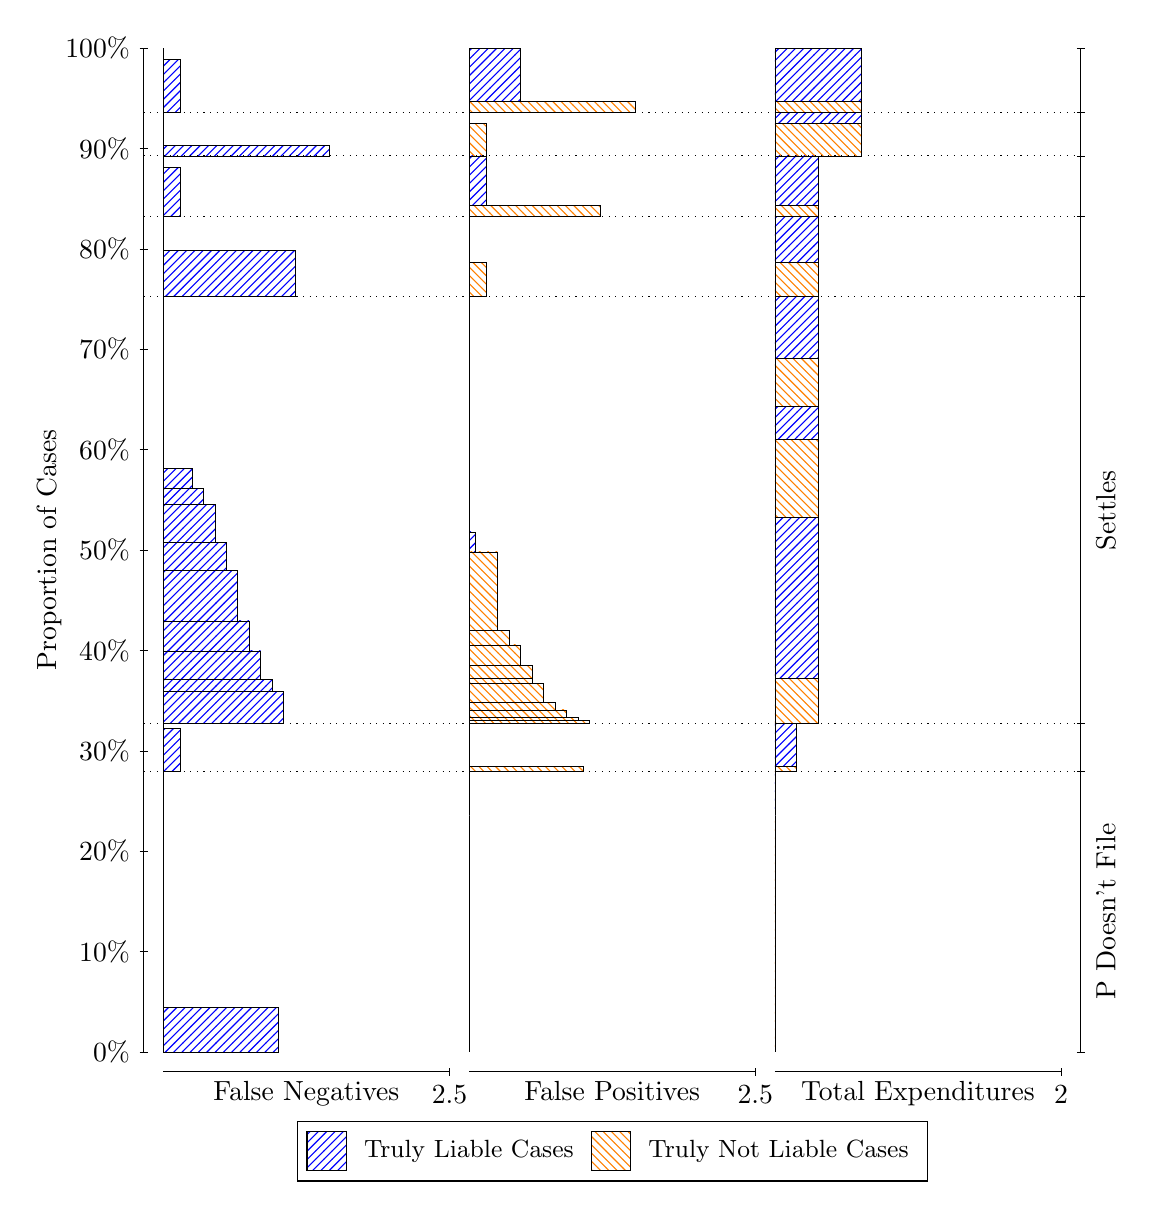
\begin{tikzpicture}
\draw[black, very thin] (1.5,1.75) -- (1.5,14.5);
\node[rotate=90, text=black, anchor=center] at (0.3, 8.125) {Proportion of Cases};
\draw[black, very thin] (1.45,1.75) -- (1.55,1.75);
\node[text=black, anchor=east] at (1.45, 1.75) {0\%};
\draw[black, very thin] (1.45,3.025) -- (1.55,3.025);
\node[text=black, anchor=east] at (1.45, 3.025) {10\%};
\draw[black, very thin] (1.45,4.3) -- (1.55,4.3);
\node[text=black, anchor=east] at (1.45, 4.3) {20\%};
\draw[black, very thin] (1.45,5.575) -- (1.55,5.575);
\node[text=black, anchor=east] at (1.45, 5.575) {30\%};
\draw[black, very thin] (1.45,6.85) -- (1.55,6.85);
\node[text=black, anchor=east] at (1.45, 6.85) {40\%};
\draw[black, very thin] (1.45,8.125) -- (1.55,8.125);
\node[text=black, anchor=east] at (1.45, 8.125) {50\%};
\draw[black, very thin] (1.45,9.4) -- (1.55,9.4);
\node[text=black, anchor=east] at (1.45, 9.4) {60\%};
\draw[black, very thin] (1.45,10.675) -- (1.55,10.675);
\node[text=black, anchor=east] at (1.45, 10.675) {70\%};
\draw[black, very thin] (1.45,11.95) -- (1.55,11.95);
\node[text=black, anchor=east] at (1.45, 11.95) {80\%};
\draw[black, very thin] (1.45,13.225) -- (1.55,13.225);
\node[text=black, anchor=east] at (1.45, 13.225) {90\%};
\draw[black, very thin] (1.45,14.5) -- (1.55,14.5);
\node[text=black, anchor=east] at (1.45, 14.5) {100\%};

\draw[black, very thin] (13.4,1.75) -- (13.4,14.5);
\draw[black, very thin] (13.35,1.75) -- (13.45,1.75);
\node[anchor=west] at (13.35, 1.75) {};
\draw[black, very thin] (13.35,5.3169) -- (13.45,5.3169);
\node[anchor=west] at (13.35, 5.3169) {};
\draw[black, very thin] (13.35,5.9186) -- (13.45,5.9186);
\node[anchor=west] at (13.35, 5.9186) {};
\draw[black, very thin] (13.35,11.342) -- (13.45,11.342);
\node[anchor=west] at (13.35, 11.342) {};
\draw[black, very thin] (13.35,12.361) -- (13.45,12.361);
\node[anchor=west] at (13.35, 12.361) {};
\draw[black, very thin] (13.35,13.13) -- (13.45,13.13);
\node[anchor=west] at (13.35, 13.13) {};
\draw[black, very thin] (13.35,13.684) -- (13.45,13.684);
\node[anchor=west] at (13.35, 13.684) {};
\draw[black, very thin] (13.35,14.5) -- (13.45,14.5);
\node[anchor=west] at (13.35, 14.5) {};

\draw[black, very thin, pattern color=blue, pattern=north east lines] (1.75,1.75) rectangle (3.2033,2.3168);
\draw[black, very thin, pattern color=orange, pattern=north west lines] (1.75,2.3168) rectangle (1.75,5.3169);
\draw[black, very thin, pattern color=blue, pattern=north east lines] (1.75,5.3169) rectangle (1.968,5.8597);
\draw[black, very thin, pattern color=orange, pattern=north west lines] (1.75,5.8597) rectangle (1.75,5.9186);
\draw[black, very thin, pattern color=blue, pattern=north east lines] (1.75,5.9186) rectangle (3.276,6.3299);
\draw[black, very thin, pattern color=blue, pattern=north east lines] (1.75,6.3299) rectangle (3.1307,6.4783);
\draw[black, very thin, pattern color=blue, pattern=north east lines] (1.75,6.4783) rectangle (2.9853,6.8444);
\draw[black, very thin, pattern color=blue, pattern=north east lines] (1.75,6.8444) rectangle (2.84,7.2244);
\draw[black, very thin, pattern color=blue, pattern=north east lines] (1.75,7.2244) rectangle (2.6947,7.8691);
\draw[black, very thin, pattern color=blue, pattern=north east lines] (1.75,7.8691) rectangle (2.5493,8.226);
\draw[black, very thin, pattern color=blue, pattern=north east lines] (1.75,8.226) rectangle (2.404,8.7001);
\draw[black, very thin, pattern color=blue, pattern=north east lines] (1.75,8.7001) rectangle (2.2587,8.904);
\draw[black, very thin, pattern color=blue, pattern=north east lines] (1.75,8.904) rectangle (2.1133,9.1579);
\draw[black, very thin, pattern color=orange, pattern=north west lines] (1.75,9.1579) rectangle (1.75,11.342);
\draw[black, very thin, pattern color=blue, pattern=north east lines] (1.75,11.342) rectangle (3.4213,11.928);
\draw[black, very thin, pattern color=orange, pattern=north west lines] (1.75,11.928) rectangle (1.75,12.361);
\draw[black, very thin, pattern color=blue, pattern=north east lines] (1.75,12.361) rectangle (1.968,12.987);
\draw[black, very thin, pattern color=orange, pattern=north west lines] (1.75,12.987) rectangle (1.75,13.13);
\draw[black, very thin, pattern color=blue, pattern=north east lines] (1.75,13.13) rectangle (3.8573,13.268);
\draw[black, very thin, pattern color=orange, pattern=north west lines] (1.75,13.268) rectangle (1.75,13.684);
\draw[black, very thin, pattern color=blue, pattern=north east lines] (1.75,13.684) rectangle (1.968,14.36);
\draw[black, very thin, pattern color=orange, pattern=north west lines] (1.75,14.36) rectangle (1.75,14.5);
\draw[black, very thin, pattern color=orange, pattern=north west lines] (5.6333,1.75) rectangle (5.6333,4.7501);
\draw[black, very thin, pattern color=blue, pattern=north east lines] (5.6333,4.7501) rectangle (5.6333,5.3169);
\draw[black, very thin, pattern color=orange, pattern=north west lines] (5.6333,5.3169) rectangle (7.0867,5.3758);
\draw[black, very thin, pattern color=blue, pattern=north east lines] (5.6333,5.3758) rectangle (5.6333,5.9186);
\draw[black, very thin, pattern color=orange, pattern=north west lines] (5.6333,5.9186) rectangle (7.1593,5.9615);
\draw[black, very thin, pattern color=orange, pattern=north west lines] (5.6333,5.9615) rectangle (7.014,6.0007);
\draw[black, very thin, pattern color=orange, pattern=north west lines] (5.6333,6.0007) rectangle (6.8687,6.0933);
\draw[black, very thin, pattern color=orange, pattern=north west lines] (5.6333,6.0933) rectangle (6.7233,6.1857);
\draw[black, very thin, pattern color=orange, pattern=north west lines] (5.6333,6.1857) rectangle (6.578,6.4346);
\draw[black, very thin, pattern color=orange, pattern=north west lines] (5.6333,6.4346) rectangle (6.4327,6.4915);
\draw[black, very thin, pattern color=orange, pattern=north west lines] (5.6333,6.4915) rectangle (6.4327,6.6607);
\draw[black, very thin, pattern color=orange, pattern=north west lines] (5.6333,6.6607) rectangle (6.2873,6.9211);
\draw[black, very thin, pattern color=orange, pattern=north west lines] (5.6333,6.9211) rectangle (6.142,7.1059);
\draw[black, very thin, pattern color=orange, pattern=north west lines] (5.6333,7.1059) rectangle (5.9967,8.1023);
\draw[black, very thin, pattern color=blue, pattern=north east lines] (5.6333,8.1023) rectangle (5.706,8.3562);
\draw[black, very thin, pattern color=blue, pattern=north east lines] (5.6333,8.3562) rectangle (5.6333,11.342);
\draw[black, very thin, pattern color=orange, pattern=north west lines] (5.6333,11.342) rectangle (5.8513,11.775);
\draw[black, very thin, pattern color=blue, pattern=north east lines] (5.6333,11.775) rectangle (5.6333,12.361);
\draw[black, very thin, pattern color=orange, pattern=north west lines] (5.6333,12.361) rectangle (7.3047,12.504);
\draw[black, very thin, pattern color=blue, pattern=north east lines] (5.6333,12.504) rectangle (5.8513,13.13);
\draw[black, very thin, pattern color=orange, pattern=north west lines] (5.6333,13.13) rectangle (5.8513,13.545);
\draw[black, very thin, pattern color=blue, pattern=north east lines] (5.6333,13.545) rectangle (5.6333,13.684);
\draw[black, very thin, pattern color=orange, pattern=north west lines] (5.6333,13.684) rectangle (7.7407,13.824);
\draw[black, very thin, pattern color=blue, pattern=north east lines] (5.6333,13.824) rectangle (6.2873,14.5);
\draw[black, very thin, pattern color=orange, pattern=north west lines] (9.5167,1.75) rectangle (9.5167,4.7501);
\draw[black, very thin, pattern color=blue, pattern=north east lines] (9.5167,4.7501) rectangle (9.5167,5.3169);
\draw[black, very thin, pattern color=orange, pattern=north west lines] (9.5167,5.3169) rectangle (9.7892,5.3758);
\draw[black, very thin, pattern color=blue, pattern=north east lines] (9.5167,5.3758) rectangle (9.7892,5.9186);
\draw[black, very thin, pattern color=orange, pattern=north west lines] (9.5167,5.9186) rectangle (10.062,6.4915);
\draw[black, very thin, pattern color=blue, pattern=north east lines] (9.5167,6.4915) rectangle (10.062,8.5364);
\draw[black, very thin, pattern color=orange, pattern=north west lines] (9.5167,8.5364) rectangle (10.062,9.5328);
\draw[black, very thin, pattern color=blue, pattern=north east lines] (9.5167,9.5328) rectangle (10.062,9.944);
\draw[black, very thin, pattern color=orange, pattern=north west lines] (9.5167,9.944) rectangle (10.062,10.558);
\draw[black, very thin, pattern color=blue, pattern=north east lines] (9.5167,10.558) rectangle (10.062,11.342);
\draw[black, very thin, pattern color=orange, pattern=north west lines] (9.5167,11.342) rectangle (10.062,11.775);
\draw[black, very thin, pattern color=blue, pattern=north east lines] (9.5167,11.775) rectangle (10.062,12.361);
\draw[black, very thin, pattern color=orange, pattern=north west lines] (9.5167,12.361) rectangle (10.062,12.504);
\draw[black, very thin, pattern color=blue, pattern=north east lines] (9.5167,12.504) rectangle (10.062,13.13);
\draw[black, very thin, pattern color=orange, pattern=north west lines] (9.5167,13.13) rectangle (10.607,13.545);
\draw[black, very thin, pattern color=blue, pattern=north east lines] (9.5167,13.545) rectangle (10.607,13.684);
\draw[black, very thin, pattern color=orange, pattern=north west lines] (9.5167,13.684) rectangle (10.607,13.824);
\draw[black, very thin, pattern color=blue, pattern=north east lines] (9.5167,13.824) rectangle (10.607,14.5);
\draw[black, dotted] (1.5,5.3169) -- (13.4,5.3169);
\draw[black, dotted] (1.5,5.9186) -- (13.4,5.9186);
\draw[black, dotted] (1.5,11.342) -- (13.4,11.342);
\draw[black, dotted] (1.5,12.361) -- (13.4,12.361);
\draw[black, dotted] (1.5,13.13) -- (13.4,13.13);
\draw[black, dotted] (1.5,13.684) -- (13.4,13.684);
\draw[black, very thin] (1.75,1.5) -- (5.3833,1.5);
\node[text=black, anchor=north] at (3.5667, 1.5) {False Negatives};
\draw[black, very thin] (5.3833,1.45) -- (5.3833,1.55);
\node[text=black, anchor=north] at (5.3833, 1.45) {2.5};

\draw[black, very thin] (5.6333,1.5) -- (9.2667,1.5);
\node[text=black, anchor=north] at (7.45, 1.5) {False Positives};
\draw[black, very thin] (9.2667,1.45) -- (9.2667,1.55);
\node[text=black, anchor=north] at (9.2667, 1.45) {2.5};

\draw[black, very thin] (9.5167,1.5) -- (13.15,1.5);
\node[text=black, anchor=north] at (11.333, 1.5) {Total Expenditures};
\draw[black, very thin] (13.15,1.45) -- (13.15,1.55);
\node[text=black, anchor=north] at (13.15, 1.45) {2};

\node[text=black, centered, rotate=90] at (13.72, 3.5334) {P Doesn't File};

\node[text=black, centered, rotate=90] at (13.72, 8.6301) {Settles};





\draw (7.449999999999999,1.5) node[draw=none] (baseCoordinate) {};
\begin{scope}[align=center]
        \matrix[scale=0.5, draw=black, below=0.5cm of baseCoordinate, nodes={draw}, column sep=0.1cm]{
            \node[rectangle, draw, minimum width=0.5cm, minimum height=0.5cm, pattern color=blue, pattern=north east lines] {}; &
            \node[draw=none, font=\small, text=black] (B) {Truly Liable Cases}; &
            \node[rectangle, draw, minimum width=0.5cm, minimum height=0.5cm, pattern color=orange, pattern=north west lines] {}; &
            \node[draw=none, font=\small, text=black] (B) {Truly Not Liable Cases}; \\
            };
\end{scope}

\end{tikzpicture}
\end{document}